\section{Experiment 2: simulated data with latent structure}

In the second simulation experiment, we generated data from a confirmatory factor analysis (CFA) model.
The data social scientists analyze often comprise items measuring different latent constructs, 
a characteristic that is likely to impact imputation performance.
In Experiment 2, we varied three design factors: dimensionality of the data, size of the factor loadings, and proportion of missing data.
We controlled the dimensionality of the data by the number of latent variables, $l \in \{10, 100\}$.
We generated five items to measure each latent variable, resulting in either 50 or 500 total items. We held the sample size constant at $n=200$, so conditions with $l = 10$ resulted in a low-dimensional data, while conditions 
with $l = 100$ resulted in high-dimensional data.
We defined the factor loadings as a two-level random factor.
We sampled the high factor loadings from Unif(0.9, 0.97), and we sampled the low factor loadings from Unif(0.5, 0.6).
We defined the proportion of missing values as either $pm = 0.1$ or $pm = 0.3$.
Table \ref{tab:condExp2} summarizes the eight resulting conditions. We conducted $S = 1000$ replications of each condition. For each replicate, missing values were imposed, and then each of the missing data treatments used in Experiment 1 was used to obtain estimates of the parameters of a the analysis models described below.

\begin{table}
\tbl{Summary of conditions for Experiment 2.}
	{
	\begin{tabular}{l c c c c c c } 
		\toprule
		condition & label & n & p & l & pm & $\lambda$ range \\
		\midrule
		1 & low-dim-low-pm-high-$\lambda$ & 200 & 50 &  10 &  0.1 & [0.9, 0.97] \\
		2 & high-dim-low-pm-high-$\lambda$ & 200 & 500 & 100 & 0.1 & [0.9, 0.97] \\
		3 & low-dim-high-pm-high-$\lambda$ & 200 & 50 &  10 &  0.3 & [0.9, 0.97] \\
		4 & high-dim-high-pm-high-$\lambda$ & 200 & 500 & 100 & 0.3 & [0.9, 0.97] \\
		5 & low-dim-low-pm-low-$\lambda$ & 200 & 50 &  10 &  0.1 & [0.5, 0.6]  \\
		6 & high-dim-low-pm-low-$\lambda$ & 200 & 500 & 100 & 0.1 & [0.5, 0.6]  \\
		7 & low-dim-high-pm-low-$\lambda$ & 200 & 50 &  10 &  0.3 & [0.5, 0.6]  \\
		8 & high-dim-high-pm-low-$\lambda$ & 200 & 500 & 100 & 0.3 & [0.5, 0.6]  \\
		\bottomrule
	\end{tabular}
	}
\label{tab:condExp2}
\end{table}

\FloatBarrier % stops table:condSum leaving its own section

\subsection{Simulation study procedure}

\subsubsection{Data generation}
	For each replication, we created an $n \times p$ data matrix, $\bm{Z}$, based on a CFA model.
	Each of $l$ latent variables was measured by five items, for a total of $p = 5*l$ 
	columns in $\bm{Z}$.
	Values of the items for the $i$th observation were generated with the following measurement model:
%
	\begin{equation}
		\bm{z}_i = \bm{\Lambda} \bm{\xi}_i + \bm{\delta}_i
	\end{equation}
%
	where $\bm{z}_i$ is a vector of $5*l$ item scores for observation $i = 1, ..., n$;
	$\bm{\Lambda}$ is the $(5*l) \times l$ matrix of factor loadings; $\bm{\xi}_i$ is a vector of $l$ latent variable scores 
	for observation $i$, and $\bm{\delta}_i$ is a vector of $5*l$ measurement errors sampled from a 
	multivariate normal distribution with means of zero and a diagonal covariance matrix, $\bm{\Theta}$.
	We rescaled all items to have means of five.
	For notation and model specification, the interested reader may refer to \cite{bollen:1989}.

	We sampled the latent scores in $\bm{\xi}_i$ from a multivariate normal distribution with means of zero and covariance matrix $\bm{\Psi}$. We defined the off-diagonal elements of $\bm{\Psi}$ such that the first four latent variables were highly correlated ($\rho = 0.6$), the second block of four 
	latent variables were weakly correlated ($\rho = 0.3$), and the remaining $l-8$ latent variables were uncorrelated.

	$\bm{\Lambda}$ defined a simple latent structure where each item loaded onto only one factor.
	Both the item and latent factor variances were set to 1, so the measurement error variance was defined as 
	$var(\delta) = 1 - \lambda^{2}$.
	This specification allowed the factor loadings to be
	interpreted as standardized values between 0 and 1.
	For each repetition, we sampled the exact values of the factor loadings from a uniform distribution with bounds defined by the condition.

\subsubsection{Missing data imposition}

	Item nonresponse was imposed on 10 items in $\bm{Z}$ using Equation \eqref{eqn:rm} to define the probability
	of nonresponse.
	The indicators of the first two highly correlated latent variables
	($l = \{1, 2\}$) were candidates for missing data imposition.
The latent scores for the other two highly correlated latent 
	variables ($l = \{3, 4\}$) acted as the missing data predictors comprising the columns of $\tilde{\bm{Z}}$.
	
\subsubsection{Imputation}
	
	The missing values were treated with all the methods previously described.
	The imputation methods were parameterized as in Experiment 1.
	The same convergence checking procedure used in Experiment 1 suggested that 50 iterations were sufficient for convergence of all MI methods except blasso, which required approximately 
	2,000 iterations for convergence.

\subsubsection{Analysis}
	
	The substantive model of interest in Experiment 2 was a saturated model that estimated means,
	variances, and covariances of the raw items with missing values.
	Furthermore, we estimated the true CFA model for the same items to evaluate the estimation of the factor loadings.
	Results for the CFA model are reported in the supplementary material.

\subsection{Results}
	To assess the performance of the methods, we used the same comparison criteria described for Experiment 1.
	Figures \ref{fig:exp2bias14} and \ref{fig:exp2cir14} report the maximum, average, and minimum $|\text{PRB}|$ and 
	CIC obtained with each missing data treatment method for each parameter type (mean, variance, and covariance) in 
	the conditions with high factor loadings.
	Figures \ref{fig:exp2bias58} and \ref{fig:exp2cir58} report the same results for the conditions with low 
	factor loadings.
	We included figures reporting the raw PRBs and CICs for every parameter in the supplementary materials.

	\subsubsection{Means}
	All imputation methods resulted in unbiased estimates of the item means in all conditions.
	In particular, IURR, MI-PCA, and MI-OP exhibited the smallest bias, and only CC produced any meaningful 
	bias of the means. MI-PCA was the only method that produced reasonable coverages in all conditions. When $pm$ was low, all methods expect missFor and CC produced reasonable coverages, regardless of the factor loading size.
	When factor loadings were large, DURR and IURR resulted in minimal deviations from nominal 
	coverage, while blasso, bridge, MI-CART, MI-RF, and missFor led to problematic under-coverage when the $pm$ was high.
	In the conditions with lower factor loadings, all methods performed worse, but relative performances remain
	unchanged.
	IURR, MI-PCA, and MI-OP again exhibited the smallest biases and deviations from nominal coverage rates.
	However, MI-PCA and MI-OP were the only methods that produced reasonable coverage rates in the 
	high-dim-high-pm-low-$\lambda$ condition. CC produced extreme levels of under-coverage across all conditions.
	
	\subsubsection{Variances}
	
	\paragraph{High factor loadings} 
	All MI methods, except bridge, resulted in acceptable estimation bias for the item variances in the conditions
	with large factor loadings. The bridge estimates were unbiased in the low-dimensional conditions but biased in the high-dimensional conditions.
	IURR, MI-PCA, and MI-OP produced the least biased estimates, while missFor and CC tended to produce large biases.
	In the low-pm conditions, all methods expect for missFor and CC produced reasonable coverages. In the high-pm conditions, only IURR, MI-PCA, and MI-OP maintained reasonable coverages. Bridge produced good coverage in the low-dim-high-pm condition, wherein blasso and DURR produced borderline-acceptable coverages. All three methods, however, produced problematic under-coverage in the high-dim-high-pm condition. The tree-based MI methods produced extreme under-coverage whenever $pm$ was high.
	CC and missFor again showed extreme under-coverage in all conditions.
	%The large bias and low coverage for the item variances that afflicted %MI-PCA in the multivariate-normal set up 
	%(figures \ref{fig:exp1bias} and \ref{fig:exp1cir}) was not present in %the high factor loading conditions.
	%However, that pattern reappeared in the conditions with low factor %loadings (see figures \ref{fig:exp2bias58} 
	%and \ref{fig:exp2cir58}).

\paragraph{Low factor loadings}
IURR, blasso, MI-CART, MI-RF, CC, and MI-OP produced unbiased variance estimates in all low-$\lambda$ conditions. IURR, blasso, and the tree-based MI methods showed the lowest biases. Bridge produced unacceptable biases in the low-dim-high-pm condition, while DURR and MI-PCA produced large biases in the high-dim-high-pm condition. missFor tended to produce problematic biases in all conditions. Only blasso and MI-OP produced reasonable coverages in all low-$\lambda$ conditions. IURR and MI-PCA produced reasonable coverage in all but the high-dim-high-pm condition where they both led to substantial under-coverage. The tree-based MI methods produced good coverage with low $pm$ and borderline-acceptable coverages in the high-pm conditions. DURR produced extreme under-coverage in all but the low-dim-low-pm condition, while missFor and CC tended to produce problematic under-coverage in all conditions.

	\subsubsection{Covariances}
	
	As in Experiment 1, MI-PCA resulted in the lowest biases and the smallest deviations from nominal coverage. Other than MI-OP, MI-PCA was the only method that produced unbiased covariance estimates and reasonable coverages across all conditions. IURR produced unbiased estimates and acceptable to borderline-acceptable CICs in all but the high-dim-high-pm-low-$\lambda$ condition.
	For all the conditions with high factor loadings, DURR showed acceptable biases but under-covered in the high-dim-high-pm-high-$\lambda$ condition.
	However, DURR produced large covariance biases and under-coverage in all the low-$\lambda$ conditions expect for the low-dim-low-pm-low-$\lambda$ condition.
	Except in the low-pm-high-$\lambda$ conditions, all other methods tended to produce large biases and problematic degrees of under-coverage.

\begin{figure}
	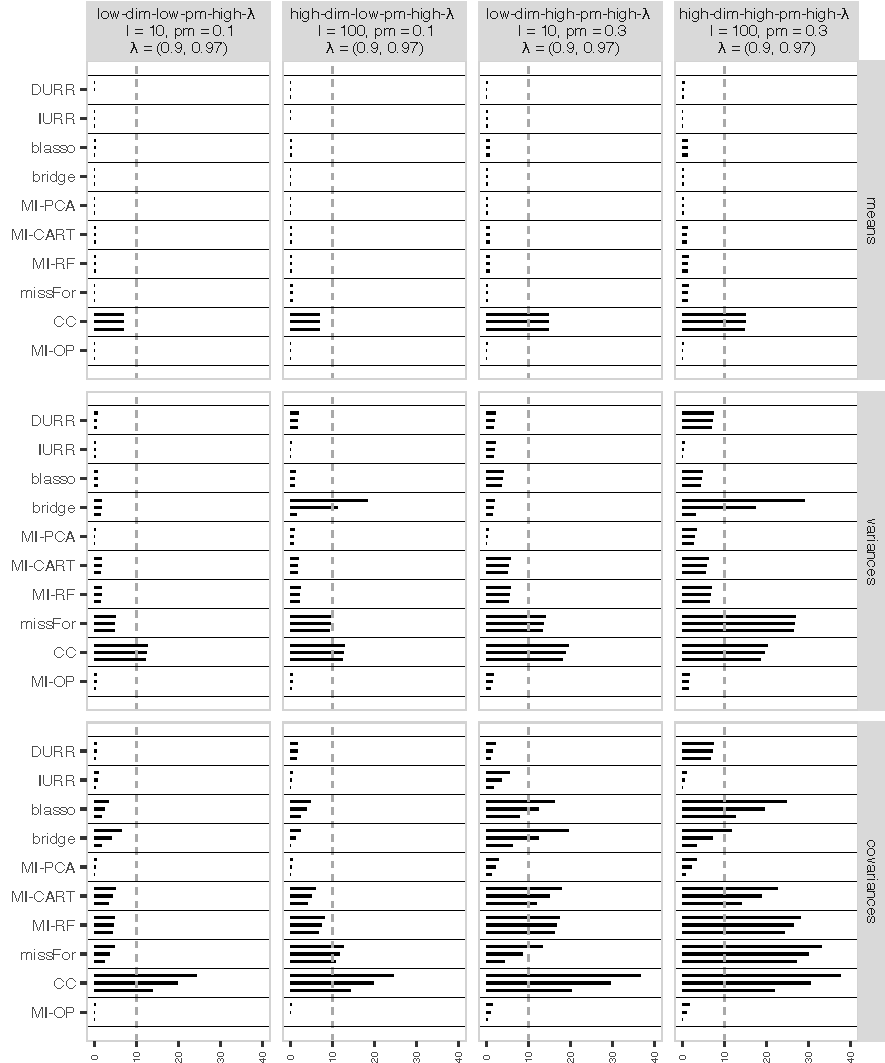
\includegraphics{\pathFIG/exp2_semR_bias_14_summy.pdf}
\caption{
	Maximum, average, and minimum absolute Percent Relative Bias ($|\text{PRB}|$) for item means, variances, 
	and covariances in the conditions of Experiment 2 with high factor loadings.
}
\label{fig:exp2bias14}
\end{figure}

\begin{figure}
	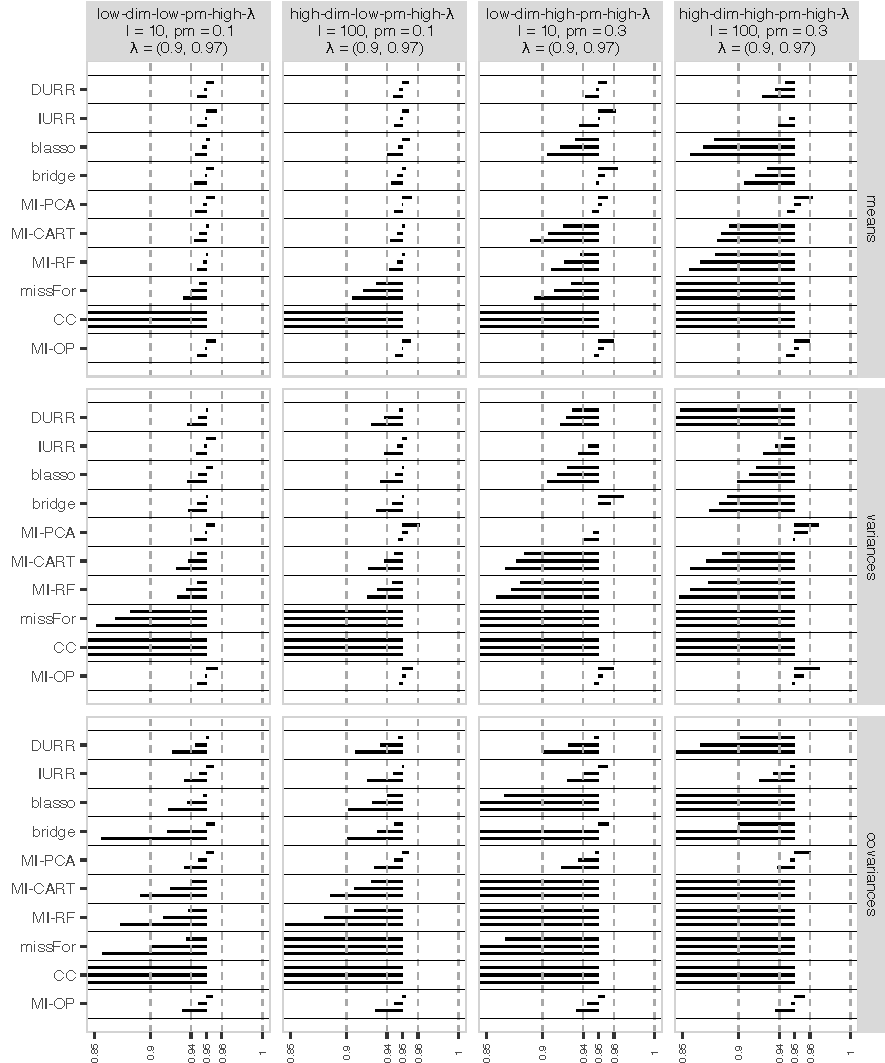
\includegraphics{\pathFIG/exp2_semR_ci_14_summy.pdf}
\caption{
	Maximum, average, and minimum CIC for item means, variances, and covariances in Experiment 2
	in the conditions of Experiment 2 with high factor loadings.
}
\label{fig:exp2cir14}
\end{figure}

\begin{figure}
	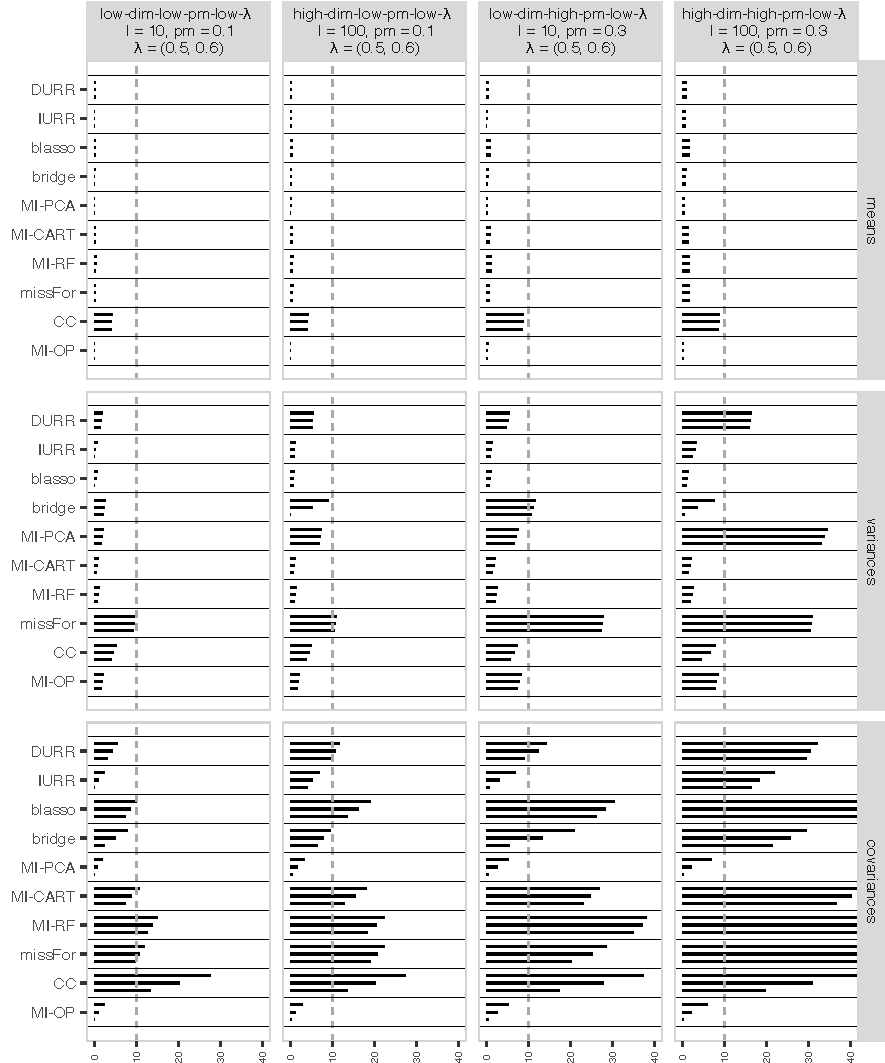
\includegraphics{\pathFIG/exp2_semR_bias_58_summy.pdf}
\caption{
	Maximum, average, and minimum absolute Percent Relative Bias ($|\text{PRB}|$) for item means, variances, 
	and covariances in the conditions of Experiment 2 with low factor loadings.
}
\label{fig:exp2bias58}
\end{figure}

\begin{figure}
	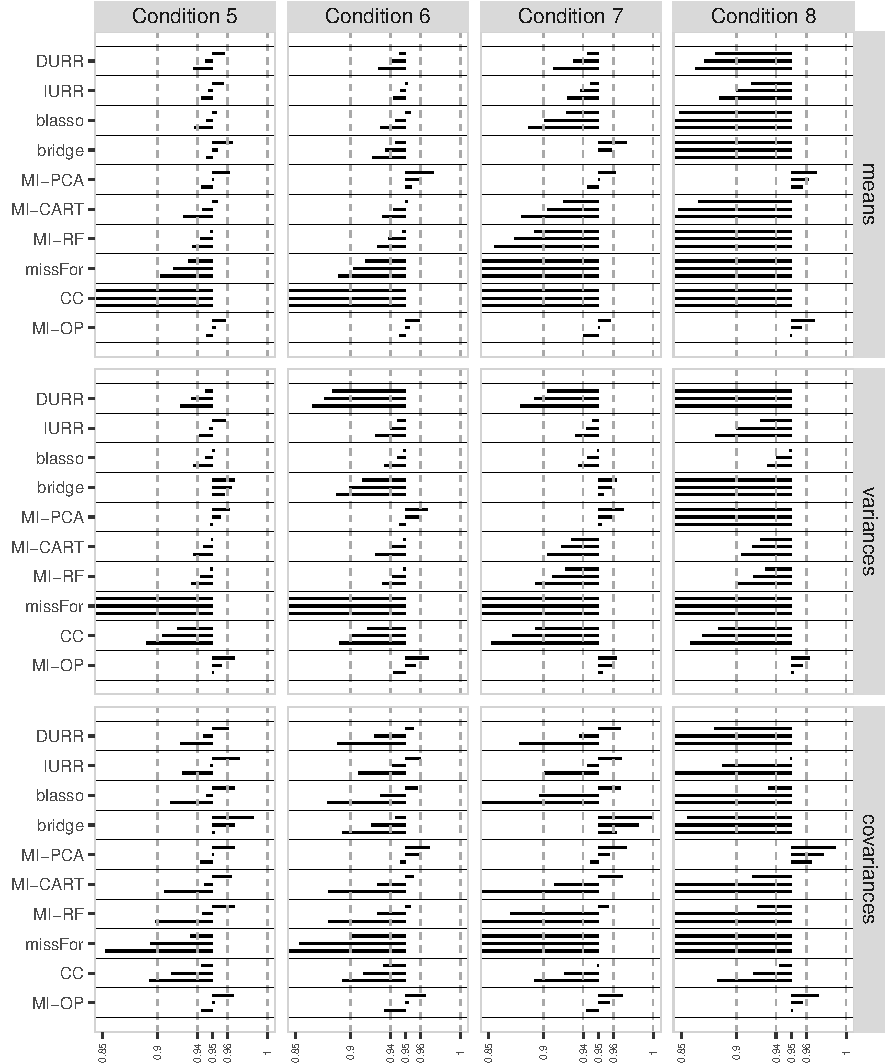
\includegraphics{\pathFIG/exp2_semR_ci_58_summy.pdf}
\caption{
	Maximum, average, and minimum CIC for item means, variances, and covariances in the conditions of 
	Experiment 2 with low factor loadings.
}
\label{fig:exp2cir58}
\end{figure}

\FloatBarrier

